\documentclass[border=0.8ex,svgnames,tikz]{standalone}
\usepackage{amsmath,mathtools}
\usepackage{fontspec}
\setmainfont{Source Serif 4}
\setsansfont{Source Sans 3}
\setmonofont{Source Code Pro}

\usetikzlibrary{chains,calc}

\begin{document}
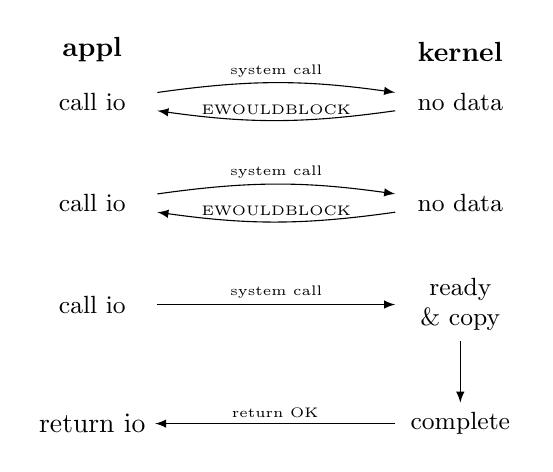
\begin{tikzpicture}[node distance=3em]
  \coordinate(appl) at (0,0);
  \coordinate(kernel) at ($(appl)+(13.3em,0)$);
  \begin{scope}[
    every node/.style={
      on chain,
      align=center,
      anchor=center,
      font=\small,
      text width=4em,
    },
    start chain=going below,
    ]
    \chainin(kernel);
    \node (noready1) {no data};
    \node (noready2) {no data};
    \node (ready)    {ready \& copy};
    \node (complete) {complete};
  \end{scope}
  \begin{scope}[
    every node/.style={
      on chain,
      align=center,
      anchor=center,
      font=\small,
      text width=4em,
    },
    start chain=going below,
    ]
    \chainin(appl);
    \node (call1)  {call io};
    \node (call2)  {call io};
    \node (call3)  {call io};
  \end{scope}
  \node (return) at ($(call3)+(complete)-(ready)$) {return io};
  \begin{scope}[
    every node/.style={above,font=\tiny,inner sep=0.45ex},
    every path/.style={draw,>=latex},
    ]
    \path[->]
    (call1)    edge[bend left=8] node{system call}  (noready1)
    (noready1) edge[bend left=8] node{EWOULDBLOCK}  (call1)
    (call2)    edge[bend left=8] node{system call}  (noready2)
    (noready2) edge[bend left=8] node{EWOULDBLOCK}  (call2)
    (call3)    edge               node{system call} (ready)
    (ready)    edge                                 (complete)
    (complete) edge               node{return OK}   (return);
  \end{scope}
  \node[above=1ex of call1]{\bfseries appl};
  \node[above=1ex of noready1]{\bfseries kernel};
\end{tikzpicture}
\end{document}
